% Vektorgrafiken ausschließlich für die Lesefassung.
% Benötigt TikZ ohne zusätzliche Bibliotheken.
\definecolor{semilatticeblue}{RGB}{34,92,133}
\definecolor{semilatticeshade}{RGB}{226,237,244}

\newcommand{\SemilatticeExampleDiagram}{%
  \par\medskip\noindent
  \begin{minipage}{\linewidth}
  \centering
  \begin{minipage}[c]{.57\linewidth}
    \centering\small
    \textbf{Die Vereinigungstafel}\par\medskip
    \begingroup
    \setlength{\tabcolsep}{5pt}
    \renewcommand{\arraystretch}{1.5}
    \begin{tabular}{c|cccc}
      \(\cup\) & \(\varnothing\) & \(\{a\}\) & \(\{b\}\) & \(S\)\\\hline
      \(\varnothing\) & \(\varnothing\) & \(\{a\}\) & \(\{b\}\) & \(S\)\\
      \(\{a\}\) & \(\{a\}\) & \(\{a\}\) & \(S\) & \(S\)\\
      \(\{b\}\) & \(\{b\}\) & \(S\) & \(\{b\}\) & \(S\)\\
      \(S\) & \(S\) & \(S\) & \(S\) & \(S\)
    \end{tabular}
    \endgroup
  \end{minipage}\hfill
  \begin{minipage}[c]{.39\linewidth}
    \centering\small
    \textbf{Die Inklusionsordnung}\par\smallskip
    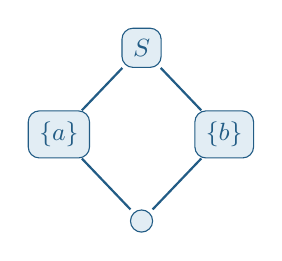
\begin{tikzpicture}[x=1cm,y=1cm,font=\small,
      subset/.style={draw=semilatticeblue,fill=semilatticeshade,
        rounded corners,inner sep=4pt,text=semilatticeblue}]
      \node[subset] (empty) at (0,0) {\(\varnothing\)};
      \node[subset] (a) at (-1.05,1.1) {\(\{a\}\)};
      \node[subset] (b) at (1.05,1.1) {\(\{b\}\)};
      \node[subset] (full) at (0,2.2) {\(S\)};
      \draw[thick,semilatticeblue] (empty)--(a)--(full)
        (empty)--(b)--(full);
    \end{tikzpicture}
  \end{minipage}
  \par\medskip\small\raggedright
  Hier ist \(S=\{a,b\}\) mit \(a\neq b\). Links steht im Feld
  der Zeile \(X\) und der Spalte \(Y\) das Ergebnis \(X\cup Y\).
  Rechts verläuft die Ordnung von unten nach oben. Aufsteigende Wege
  stehen für echte Inklusionen; die reflexiven Vergleiche werden
  im Hasse-Diagramm nicht eingezeichnet.
  \end{minipage}\par\medskip
}

\newcommand{\SemilatticeCorrespondenceDiagram}{%
  \par\medskip\noindent
  \begin{minipage}{\linewidth}
  \centering
  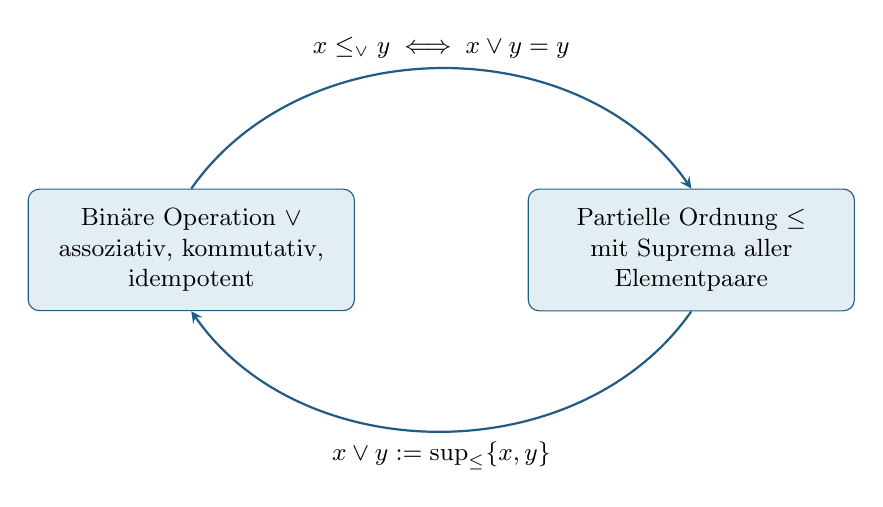
\begin{tikzpicture}[x=1cm,y=1cm,font=\small,>=stealth,
    description/.style={draw=semilatticeblue,fill=semilatticeshade,
      rounded corners,align=center,minimum height=1.1cm,
      text width=3.65cm,inner sep=7pt}]
    \node[description] (operation) at (0,0)
      {Binäre Operation \(\vee\)\\
       assoziativ, kommutativ,\\idempotent};
    \node[description] (order) at (6.35,0)
      {Partielle Ordnung \(\leq\)\\
       mit Suprema aller\\Elementpaare};
    \draw[->,thick,semilatticeblue]
      (operation.north) to[out=55,in=125]
      node[above,text=black] {\(x\leq_\vee y\;\Longleftrightarrow\;x\vee y=y\)}
      (order.north);
    \draw[->,thick,semilatticeblue]
      (order.south) to[out=235,in=305]
      node[below,text=black] {\(x\vee y:=\sup_{\leq}\{x,y\}\)}
      (operation.south);
  \end{tikzpicture}
  \par\medskip\small\raggedright
  Beide Übergänge behalten die Menge \(A\) bei. Geht man einmal
  im Kreis, erhält man dieselbe Operation beziehungsweise dieselbe
  Ordnung zurück. Dies ist eine Gleichheit auf dem ursprünglichen
  Träger, keine bloße Ähnlichkeit zweier Beispiele.
  \end{minipage}\par\medskip
}
